\documentclass[12pt, a4paper, twoside]{book}

\usepackage{helvet}
\usepackage{hyperref}
\usepackage{graphicx}
\usepackage{listings}
\usepackage{textcomp}
\usepackage[
	a4paper,
	outer=2cm,
	inner=4cm,
	top=2cm,
	bottom=2cm
]{geometry}
\usepackage{float}
\usepackage{tabularx}
\usepackage[disable]{todonotes}
\usepackage{color, soul}
\usepackage{amsmath}
\usepackage{algorithmicx}
\usepackage[noend]{algpseudocode}
\usepackage{algorithm}
\usepackage{framed}
\usepackage{subcaption}
\usepackage{titlepic}
\usepackage{fancyhdr}
\usepackage[simplified]{styles/pgf-umlcd}
\usepackage{shorttoc}
\usepackage{url}
\usepackage{paralist}
\usepackage{dirtytalk}

\definecolor{grey}{rgb}{0.9, 0.9, 0.9}
\definecolor{dkgreen}{rgb}{0,0.6,0}
\definecolor{dkred}{rgb}{0.6,0,0.0}

\lstdefinestyle{DOS}
{
    backgroundcolor=\color{black},
    basicstyle=\scriptsize\color{white}\ttfamily,
    stringstyle=\color{white},
    keywords={}
}

\lstdefinestyle{makefile}
{
    numberblanklines=false,
    language=make,
    tabsize=4,
    keywordstyle=\color{red},
    identifierstyle= %plain identifiers for make
}

\lstset{
  language=Python,                % the language of the code
  escapeinside={\%*}{*)},
  basicstyle=\footnotesize\ttfamily,
  numbers=left,                   % where to put the line-numbers
  stepnumber=1,                   % the step between two line-numbers. If it's 1, each line
  numbersep=5pt,                  % how far the line-numbers are from the code
  backgroundcolor=\color{white},      % choose the background color. You must add \usepackage{color}
  showspaces=false,               % show spaces adding particular underscores
  showstringspaces=false,         % underline spaces within strings
  showtabs=false,                 % show tabs within strings adding particular underscores
  frame=single,                   % adds a frame around the code
  rulecolor=\color{black},        % if not set, the frame-color may be changed on line-breaks within not-black text (e.g. comments (green here))
  tabsize=2,                      % sets default tabsize to 2 spaces
  captionpos=b,                   % sets the caption-position to bottom
  breaklines=true,                % sets automatic line breaking
  breakatwhitespace=false,        % sets if automatic breaks should only happen at whitespace
  keywordstyle=\color{blue},          % keyword style
  commentstyle=\color{dkgreen},       % comment style
  stringstyle=\color{dkred},         % string literal style
  columns=fixed,
  extendedchars=true,
  frame=single,
}

%\renewcommand{\chaptername}{Topic}

% New definitions
\algnewcommand\algorithmicswitch{\textbf{switch}}
\algnewcommand\algorithmiccase{\textbf{case}}
\algnewcommand\algorithmicassert{\texttt{assert}}
\algnewcommand\Assert[1]{\State \algorithmicassert(#1)}%
% New "environments"
\algdef{SE}[SWITCH]{Switch}{EndSwitch}[1]{\algorithmicswitch\ #1\ \algorithmicdo}{\algorithmicend\ \algorithmicswitch}%
\algdef{SE}[CASE]{Case}{EndCase}[1]{\algorithmiccase\ #1}{\algorithmicend\ \algorithmiccase}%
\algtext*{EndSwitch}%
\algtext*{EndCase}%

\pagestyle{fancy}
\fancyhf{}
\fancyhead[RO, LE]{\small \rightmark}
\fancyfoot[RO, LE]{\small \thepage}

\newcommand{\blank}[1]{\hspace*{#1}}

\begin{document}

\frontmatter

\begin{titlepage}
\vspace*{5cm}
\begin{center}

\includegraphics[width=.5\textwidth]{images/EdNapUniLogoCMYK}~\\[1cm]

\textsc{\Large Edinburgh Napier University}\\[1.5cm]

\textsc{\LARGE \bfseries SET09103 Advanced Web Technologies}\\[0.5cm]

\hrulefill \\[0.4cm]
{\huge \bfseries Notes \& Workbook 2015-2016 \\[0.4cm] }
\hrulefill \\[1.5cm]

\begin{minipage}{0.4\textwidth}
\begin{flushleft} \large
\textbf{Dr Simon Wells} \\
\end{flushleft}
\end{minipage}

\vfill

\end{center}
\end{titlepage}

\shorttoc{Overview}{0}

\setcounter{tocdepth}{2}
\cleardoublepage
\tableofcontents
\listoffigures
%\listofalgorithms
\addtocontents{toc}{~\hfill\textbf{Page}\par}

\mainmatter
%\part{Admin}

%\part{Notes}


\part{Labs \& Practical Work}
\chapter{Learning Environment Part \#1}
\label{lab1}
\paragraph{} Because Linux is one of the most widespread operating systems found on web-servers it makes sense for us to use a form of Linux as our learning environment on this \emph{Advanced} web technologies module. There are a lot of different versions of Linux, known as distributions or distros, and you might have heard or or even used some of them, for example, Debian or Ubuntu. Because we could spend an entire year learning about Linux we shall use a deliberately simplified version of a Linux environment which mimics many of the features found in a full Linux distibution. We shall also ignore many aspects, such as administration of Linux servers, so that we can focus on using Linux within the context of web-development. Our focus will be on the development of web-apps and an in depth investigation of what happens on the server side. That said, whilst we won't focus as much on the client, there is plenty of scope within the courseworks to put into practise your previous learning from the Web Techologies module from last year to make things pretty and provide a better user experience.

\paragraph{} There will be a number of core steps involved in getting acquinted with the learning environment:

\begin{enumerate}
\item Levinux - Our self-contained, virtualised Linux server which runs within Windows (or on OS X or even under Linux itself)
\item SSH - To enable us to connect from our Windows machine to our virtual Linux machine
\item Basic Linux Usage at the command line
\item Vim - This is our \emph{non-graphical} editor that we shall use to write our source code
\item Git - We shall use Git to store our source code and to ``hand in'' our coursework assignments
\end{enumerate}

\paragraph{} By the end of this section of the module you should be able to start Levinux (our Linux virtual server), log in to Linux using SSH, navigate around the command-line of our linux server, use Vim to edit our files, and use Git to store our files. This constitutes a core set of tools that should allow you to log into almost any Linux server, whether a very small one running on a Raspberry Pi\footnote{\url{https://www.raspberrypi.org}} or a very large one, for example the top 10 fastest supercomputers in the world all run a version of Linux\footnote{\url{http://www.top500.org/lists/2015/06/}}, and feel quite at home very quickly. I am not expecting you to achieve all of this in just a single lab session, but you should accomplish this easily within the lab \emph{and} this week's self-study time.

\begin{framed}
\textbf{IMPORTANT} It is a good habit for you to keep notes whenever you are learning a new tool or environment. I keep a textfile on my computer which also means that I can occasionally copy and paste commands if necessary. This way you won't have to immediately remember how you solved a problem but can look how you did it last time. This makes the whole process much less frustrating. It is how I learned to work with Linux and Git and I still refer to my notes every so often when trying to do something that I rarely do and can't quite remember the syntax for.
\end{framed}


\section{Levinux}
\label{levinux}
\paragraph{} Levinux\footnote{\url{http://www.levinux.com}} is a tiny Linux virtual server. It has just enough software installed so that you can learn about and get comfortable with a Linux system, but not so many tools that it becomes too daunting. It does however give you a launchpad from which to explore the wider world of Unix-style operating systems. If you get comfortable with Levinux then you shouldn't feel (too) lost trying any other Linux distribution. In fact the best introduction to Levinux and what it can do is probably that from the creator of Linux:\\


\say{The micro Linux distribution known as Levinux (download ~25 MB) is a tiny virtual Linux server that runs from USB or Dropbox with a double-click (no install or admin rights required) on Macs, Windows or Linux PCs—making it the perfect learning environment, and way to run \& keep your code safe for life! Think of it as an introduction to old-skool—more relevant now then ever as Linux/Unix gets embedded into everything, with an emphasis on an actual running Python/Flask web app that you can tear apart and do whatever you want with.}\\
{\bf Mike Levin} \hfill \url{http://mikelev.in/ux/}

\paragraph{} Because Levinux is so tiny you can run it easily, without needing to install it, just unzip and click to run. Levinux runs just like any other program on your desktop machine can run from your H: drive, in dropbox, or on a thumb drive. The system can be started by double clicking and you can move the same thumbdrive between different operating systems, e.g. between the Windows machines in the Napier labs and an OS X laptop, and run the exact same Linux environment.

\paragraph{} The magic that makes this possible is QEMU\footnote{\url{http://wiki.qemu.org/Main_Page}}, emulator software that provides a way to run virtual machines and has been important to the VirtualBox\footnote{\url{https://www.virtualbox.org}} and Android Virtual Device infrastructure\footnote{\url{https://developer.android.com/tools/devices/index.html}}.

\paragraph{} Levinux is basically, a set of scripts and programs that host a Linux install within a very lightweight virtual environment. The scripts manage how Levinux runs and enable it to run seamlessly across different host platforms (like Linux, Mac OS, and Windows). The programs include things like QEMU, mentioned earlier, and various virtual harddrives that are where the Linux system is installed. The specific Linux distribution that is used in Levinux is called `Tiny Core Linux'\footnote{\url{http://tinycorelinux.net/}} which is about 10MB in size and boots into a minimal command line Linux environment.

\paragraph{} Getting started with Levinux is fairly straightforward. Download levinux-master.zip from the Levinux website\footnote{\url{http://mikelev.in/ux/}}. The whole download should be around 25MB. Copy the zip file to somewhere where you want to store it, for example, a thumbdrive with 512MB free space is a good idea as you can then take your work away with you. Extract Levinux from the zip archive (i.e. right click and the zip archive and select ``Extract All...''. Don't just double click the archive as this will fail in interesting ways). Open the newly extract directory called levinux-master and double click the file called ``PipulateWindows'' (NB. If you are on OS X then just double-click ``Pipulate.app'' or if on Linux the run ``PipulateLinux.sh'').

\paragraph{} When Levinux runs, your operating system might tell you that your firewall has blocked certain features or ask for permission to allow access to certain features. You should grant access when asked. Levinux will now load and you should see something similar to th windows displayed in the following figure:

\begin{figure}[htb]
\centering
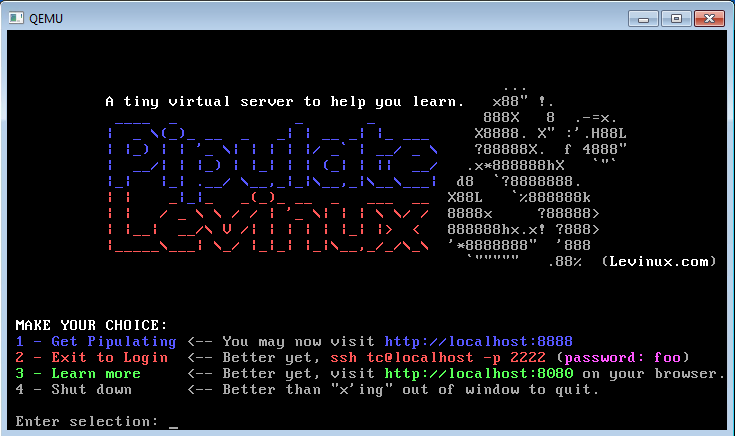
\includegraphics[width=0.75\textwidth]{images/levinux_welcome.png}
\caption{Levinux Welcome Screen}
\label{fig:levinux-welcome}
\end{figure}

\paragraph{} If you hit option 2 then you will immediately be able to log in to Levinux using the following credentials:

\begin{framed}
    \textbf{Username:} tc\blank{2cm} \textbf{Password:} foo
\end{framed}

\paragraph{} You should now see something like the following figure:

\begin{figure}[htb]
\centering
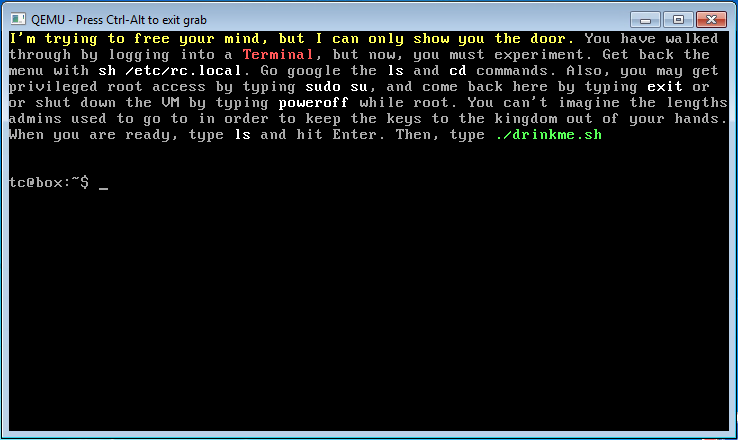
\includegraphics[width=0.75\textwidth]{images/levinux_loggedin.png}
\caption{The first screen after logging into Levinux}
\label{fig:levinux-logged-in}
\end{figure}

\paragraph{} At this point, Levinux is a minimal Linux system which has a basic set of tools but doesn't yet include any of the web development software or libraries that we will be using in this module. At this point you therefore have the option of jumping ahead to section \ref{linux} to learn a little more basic Linux, otherwise you could look at the SSH section which explains how to log in to Levinux multiple times using a tool called Secure Shell (SSH). If instead you want to get stuck in to getting your learning environment set up then you should proceed with the following steps which will install the following software:
\begin{enumerate}
\item Vim: A command-line based text editor
\item Python: A powerful programming language
\item Python-Flask: A Python library that makes it simple to build server-side web-applications
\item Various other supplementary libraries and tools that will help us to build some excellent web apps
\end{enumerate}

\paragraph{} These tools are not installed in Levinux by default because it keeps the size of the download smaller. NB. You can also install many other software packages from the Tiny Core Linux archive or from source code because this is, after all, a full Linux operating system installation. To install our extra software we do the following:

\subsection{Installing Vim}

\paragraph{} Log into Levinux if you haven't already done so then enter the following command at the prompt:
\begin{lstlisting}[style=DOS]
    tc@box:~$ ./drinkme.sh
\end{lstlisting}
\paragraph{} ./drinkme.sh runs a script that installs Vim. You will be prompted to confirm that this is what you want to do so enter `2' when asked(this might take a little while to completeas the software is being downloaded and installed into your virtual harddrive). Once the script is computer your should get your prompt back so that you can type more commands. You can launch Vim by typing `vim' at the prompt as follows (but if you are going to do that then you should probably take a look at section \ref{vim} of the notes which covers basic use of Vim):

\begin{lstlisting}[style=DOS]
    tc@box:~$ vim
\end{lstlisting}

\subsection{Installing the Web Development Environment}
\label{installing_environment}
\paragraph{} Again, if you are not logged in to Levinux then do so then enter the following command at the prompt: 

\begin{lstlisting}[style=DOS]
    tc@box:~$ sh ./Pipulate.sh 
\end{lstlisting}
\paragraph{} Again, just as for Vim, this runs a script called Pipulate.sh which installs Python, Python-Flask, a bunch of libraries, and Git. 

\paragraph{} These scripts basically sets up our development environment enabling us to edit, run, and control our source code.

\subsection{Shutting Down Levinux}
\paragraph{} The last thing we need to know about is how to safely shutdown our Levinux installation. Whilst logged in we can use the following command:
\begin{lstlisting}[style=DOS]
    tc@box:~$ sudo poweroff
\end{lstlisting}
\paragraph{} Which will cause Levinux to shutdown safely. If you are on the screen shown in figure \ref{fig:levinux-welcome} then you can just hit `4' then press $<$enter$>$. Remember, Levinux is a full computer system, even if it is running within another host system. Just as you wouldn't just hit the power button on your computer to turn it off, or at least you shouldn't, if you do that then stop it now. Instead, you should always follow the correct shut-down procedure for an operating system which gives it an opportunity to tidy itself up and clear up resources that are used. Doing anything else risks corrupting your installation so that it won't work correctly anymore and this is just as true for Levinux as it is for any other operating system.



\section{SSH}
\label{ssh}
\paragraph{} SSH which stands for `Secure Shell' is a tool for logging in to remote servers. We can use SSH to access Levinux as this provides us with an easy way to log in multiple times, e.g. have multiple shells (command lines) open and logged in to Levinux. The advantage of having multiple shells is that we can edit and save a program in one shell and run the program and monitor output in another shell. As you can imagine, this is very useful when we are developing new web apps on our Levinux server.

\paragraph{} If you are on Linux or OS X then you will already have a version of SSH installed and all you need to do is open a terminal and type the following:

\begin{lstlisting}[style=DOS]
    $ ssh tc@localhost -p 2222
\end{lstlisting}

\paragraph{} then enter the password `foo' when prompted.

\paragraph{} However if you are on Windows then your will need to download an SSH client. The most popular client for Windows is called PuTTY\footnote{\url{http://the.earth.li/~sgtatham/putty/latest/x86/putty.exe}}. Download it, put it somewhere safe where you can access it then double click it to run. There is no need to install PuTTY as it is very portable. When PuTTY runs you will be presented with the following screen:

\begin{figure}[H]
\centering
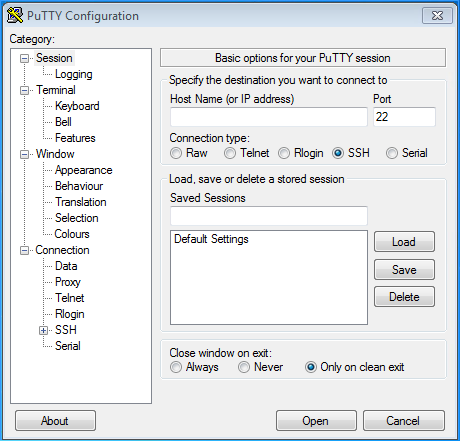
\includegraphics[width=0.5\textwidth]{images/putty_empty.png}
\caption{The PuTTY Window after you load it}
\label{fig:putty-empty}
\end{figure}

\paragraph{} You need to enter some connection details into this window as follows:

\begin{figure}[H]
\centering
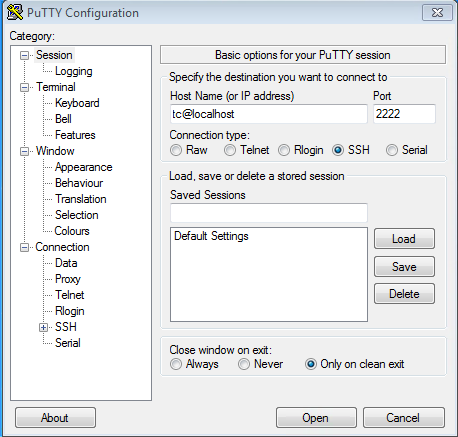
\includegraphics[width=0.5\textwidth]{images/putty_complete.png}
\caption{The PuTTY Window with completed connection details}
\label{fig:putty-complete}
\end{figure}

\paragraph{} You might be presented with the following window:

\begin{figure}[H]
\centering
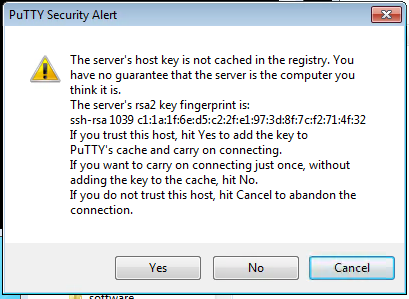
\includegraphics[width=0.5\textwidth]{images/putty_alert.png}
\caption{The PuTTY alert Window}
\label{fig:putty-alert}
\end{figure}

\paragraph{} If so, you can just click the `Yes' button. If all goes well you should now be presented with a login window for Levinux and all you have to do is type in the password (remember the password is `foo') and you should get a command line shell on your Levinux server.

\begin{figure}[H]
\centering
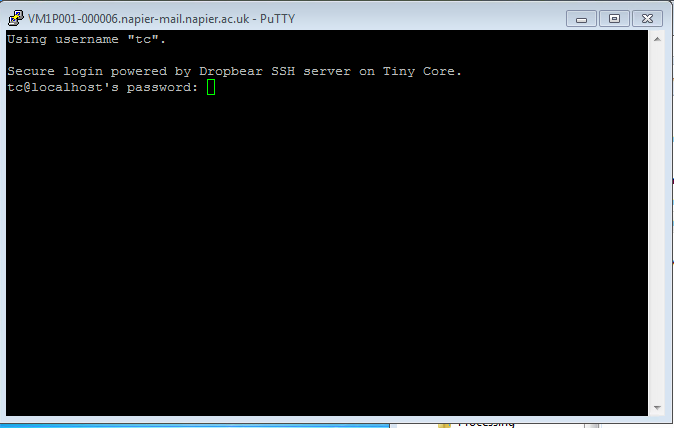
\includegraphics[width=0.75\textwidth]{images/putty_login.png}
\caption{The PuTTY login Window}
\label{fig:putty-login}
\end{figure}

\paragraph{} Remember, you can repeat this process with PuTTY as many times as required to get yourself enough shells into the Levinux server to make things easier to work with\footnote{This is not the best way to work with multiple shells. Another, more powerful way is to use a shell multiplexer, my favourite is one called Screen (\url{https://www.gnu.org/software/screen/}) but that is yet another tool to learn, and another set of commands, so lets try to keep things \emph{reasonably} simple}.


\section{Basic Linux Usage}
\label{linux}

\paragraph{} When we first log in to Linux we will see a prompt, a place where we can type commands. It looks something like this:

\begin{lstlisting}[style=DOS]
    tc@box:~$ 
\end{lstlisting}
\paragraph{} This simply means that user `tc' (short for tinycore, the default user that you logged in as) is logged into the machine called `box'. The `:' is merely a separate between the user@machine part of the prompt and the next part `{\raise.17ex\hbox{$\scriptstyle\sim$}}' which is your current location in the filesystem. The tilde or `{\raise.17ex\hbox{$\scriptstyle\sim$}}' symbol is used on Linux machines to mean your home directory.

\paragraph{} Linux has a file system, a way for all of the files that make up the running system to be organised hierarchically, just like Windows. However, on Linux the file system is organised a little differently. Instead of starting at `C:' the Linux file systems starts with `/' which is also known as the ``root'' of the filesystem. The word root is used because the Linux filesystem is shaped like a tree. All of the resources that you can access, such as your own files, are located at some level somewhere within the tree. An advantage of the Linux approach is that, when you add extra hard-drives, or mount network resources, instead of extra drive letters, all of your resources get mounted within the tree, e.g. /Volumes/Web might be the path to a remove web server and /media/cdrom might be the path to your CD-Rom drive. But other than that, from a basic user-oriented perspective, both Windows and Linux file systems are a hierarchical collection of files and directories in which any given directory might contain zero or more files or child directories.

\paragraph{} When you log in you will be located in your own directory, called your ``home'' directory which is located in the filesystem tree at 

\begin{lstlisting}[style=DOS]
    /home/tc
\end{lstlisting}
\paragraph{} You can see where you are in the filesystem by typing

\begin{lstlisting}[style=DOS]
    $ pwd
\end{lstlisting}
\paragraph{} which is short for print working directory or tell me where I am. You can type this anywhere you have a prompt. Also, no matter where you navigate to within the file system you can always return to your home directory by typing:

\begin{lstlisting}[style=DOS]
    $ cd
\end{lstlisting}

\paragraph{} You can navigate around the file system using the cd command which is short for `change directory'\footnote{You'll notice that many Linux commands are shortened versions of longer words. This is partly designed to reduce the amount of typing that you do. It may seem silly now but when you are changing directory hundreds of times a day it is much nicer to type cd than change-directory each time.}. The default version, without an argument takes you home, as we said before, but if you supply an argument then you can change the current directory. Let's try that now by changing to the root of the filesystem:

\begin{lstlisting}[style=DOS]
    $ cd /
\end{lstlisting}
\paragraph{} If you now use pwd you should see that the output is different to what it was before. You are no longer in your home directory but are in the root directory instead. Now ues the cd command without an argument to go home and use pwd to see where you are again. You can also step up through the directory hierarchy by using the `..' argument:

\begin{lstlisting}[style=DOS]
    $ cd ..
\end{lstlisting}
\paragraph{} `..' is an \emph{alias}, a label that has a default meaning, which in this case means ``move into the parent directory''. Explore the filesystem for a while using the cd, cd /, cd .., and pwd commands.

\paragraph{} There is a limit to what we can do with just these commands because we can only move into our home directory, or else navigate up through the tree to the file system root directory. We need a couple more commands to let us see what is inside a directory and to move into a new directory. For this we use the `ls' command which is short for list or list contents to see what files or child directories are in our current directory, and the cd command but with the name of a child directory as the argument. So, we can use `ls' as follows:

\begin{lstlisting}[style=DOS]
    $ ls
\end{lstlisting}

to list the files in the current directory. If you try this now you will see that your home directory contains a few default files and folders
e.g.

\begin{lstlisting}[style=DOS]
    tc@box:~$ ls
    Pipulate.sh  Recipe.sh    drinkme.sh   htdocs/
\end{lstlisting}

\paragraph{} Now we can create new files in our home directory quite easily using touch, e.g.

\begin{lstlisting}[style=DOS]
    $ touch testfile.txt
\end{lstlisting}

\paragraph{} which should give us something like this:

\begin{lstlisting}[style=DOS]
    tc@box:~$ ls
    Pipulate.sh   Recipe.sh     drinkme.sh    htdocs/       testfile.txt
\end{lstlisting}

\paragraph{} We can also create new directories using the `mkdir' which means make directory
\begin{lstlisting}[style=DOS]
    $ mkdir testdirectory
\end{lstlisting}

\paragraph{} which results in

\begin{lstlisting}[style=DOS]
    tc@box:~$ ls
    Pipulate.sh    drinkme.sh     testdirectory/
    Recipe.sh      htdocs/        testfile.txt
\end{lstlisting}
\paragraph{} We can also move files around using the `cp' and `mv' commands which are short for copy and move respectively. Let's see them in action; first we will make a copy of testfile.txt then move the copy into the testdirectory:
\begin{lstlisting}[style=DOS]
    tc@box:~$ cp testfile.txt testfile2.txt
    tc@box:~$ ls
    Pipulate.sh    drinkme.sh     testdirectory/ testfile2.txt
    Recipe.sh      htdocs/        testfile.txt
    tc@box:~$ mv testfile2.txt testdirectory/
    tc@box:~$ ls
    Pipulate.sh    drinkme.sh     testdirectory/
    Recipe.sh      htdocs/        testfile.txt
    tc@box:~$ ls testdirectory/
    testfile2.txt
\end{lstlisting}

\paragraph{} Notice that in this example we passed an argument, the name of a directory `testdirectory' to the ls command and this caused the contents of testdirectory to be listed instead of the current directory. We can do that with any directory that we have access to.

\paragraph{} Finally we might want to delete files to keep things tidy. We can use the `rm' command to remove files, e.g.
\begin{lstlisting}[style=DOS]
    tc@box:~$ rm testfile.txt 
    rm: remove 'testfile.txt'? y
    tc@box:~$ ls
    Pipulate.sh    Recipe.sh      drinkme.sh     htdocs/        testdirectory/
\end{lstlisting}
\paragraph{} We can use also use rm to remove directories, however, by default we get this behaviour:
\begin{lstlisting}[style=DOS]
    tc@box:~$ rm testdirectory/
    rm: 'testdirectory' is a directory
\end{lstlisting}
\paragraph{} What we need to do instead is to supply some options to the rm command. We need rm to act recursively, that means move into the specified directory and delete its contents and we also need to force rm not to stop and ask us for each file whether it should be deleted. We there fore need to use rm as follows:
\begin{lstlisting}[style=DOS]
    tc@box:~$ ls
    Pipulate.sh    Recipe.sh      drinkme.sh     htdocs/        testdirectory/
    tc@box:~$ rm -rf testdirectory/
    tc@box:~$ ls
    Pipulate.sh  Recipe.sh    drinkme.sh   htdocs/
\end{lstlisting}
\paragraph{} Of all the commands we have met so far, rm is the only one that can do any real damage. rm -rf could conceivably delete all of your files and directories if the command is executed in the wrong place. As a rule it is probably worth only making changes within your home directory, e.g. /home/tc, whilst working on exercises in this module, that way you are less likely to destroy your Levinux install accidentally and have to start again. However because it is easy to set up and run a new Levinux instance you can afford to experiment because if you destroy your Levniux instance you can always start again. You should however, especially once you start writing code in Levinux, keep backups of anything that you will need to use again such as the code for your courseworks.

\paragraph{} There are many, many more commands than just these. In fact you can do much more with the command line than you can with graphical tools. However, this should be enough for you to get started and is enough for you to be able to create and delete files and directories, to navigate the file system hierarchy, to list the contents of directories, and to view the contents of files. 

\paragraph{} To do more exploration of Linux, you can of course experiment with Levinux. Another good place to start is the Linux Zoo site\footnote{\url{http://www.linuxzoo.net}} which offere online virtual machines, more information, and a number of tutorials. Particularly the Linux Zoo ``essential Linux'' pages\footnote{\url{http://linuxzoo.net/page/intro.html}} which explain in more depth some of the tools that we have already covered plus many many more.








\section{Vim}
\label{vim}
\paragraph{} Vim is a command-line based text editor. It is based on an earlier editor called Vi (Vim is VI improved, hence Vim, which is a little easier to use). You might ask why we don't just use a GUI text editor like Notepad, or the editor in Visual Studio. The main reason is because we are talking about advanced web technologies, and dealing with them often involves accessing remote servers. Furthermore, the majority of servers do not have a graphical interface and only have installed the most minimal and robust set of tools. The one editor that you are almost guaranteed to find on any Unix or Linux server is Vi and by learning Vim you are well placed to handle Vi. As a result it makes sense for us to become familar with it. Many of us actually find that the shortcuts and powerful control that Vim offers us mean that we just concentrate on learning one editor very well and only use that editor rather than moving to a different editor each time we need to write a different type of document or program in a different language.

\paragraph{} What makes Vim different from many of the editors that you will be familar with, like Notepad, is that there is no role for the mouse, no buttons to click at all, only keyboard shortcuts, so we shall learn just enough of those in this module to be able to edit basic documents\footnote{However there are hundreds of Vim commands and a really clever things is that most of the commands can be chained together so that you can automate many editing tasks.}. A second very important aspect of Vim is that it is a \emph{modal} editor. When you use Vim you use it in different modes, when you are typing content into a file then you are in edit mode, and when you are entering commands you are in command mode. When Vim starts it is in command mode and anything you type will be interpreted as a command for Vim to perform. You switch into edit mode by typing `i' (for insert) and you can return to command mode at any time merely be hitting the escape key.

\begin{framed}
\textbf{IMPORTANT} If you are ever unsure what mode you are in the you can just hit escape a couple of times to ensure you are in edit mode. From here you can just type `i' again to enter the edit mode.
\end{framed}

\paragraph{} Start Vim by typing Vim at the prompt:
\begin{lstlisting}[style=DOS]
    tc@box:~$ vim
\end{lstlisting}
\paragraph{} and you will see something similar to the following:

\begin{figure}[H]
\centering
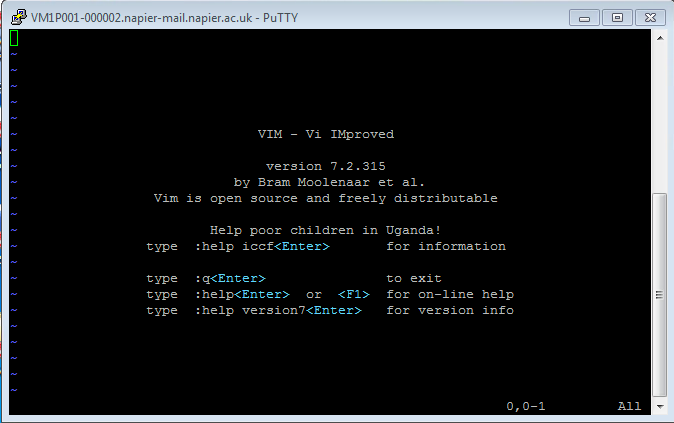
\includegraphics[width=0.75\textwidth]{images/vim_first.png}
\caption{The default Vim Editor window}
\label{fig:vim-first}
\end{figure}

\paragraph{} Let's do the easiest thing first. Let's quit Vim. To do this we enter the command mode by hitting escape then enter `:q' (where is q is short for quit) and hit enter, e.g.

\begin{lstlisting}[style=DOS]
    <ESC>:q<ENTER>
\end{lstlisting}
\paragraph{} Your Vim window should look something like this when the command is entered (but before you press enter):

\begin{figure}[H]
\centering
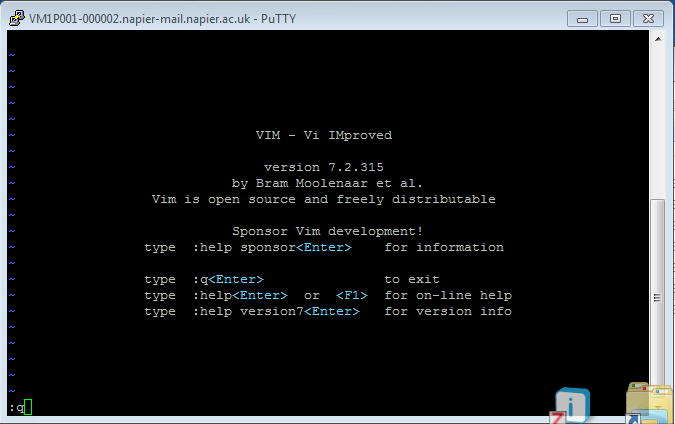
\includegraphics[width=0.75\textwidth]{images/vim_quit.png}
\caption{The Vim Editor with `:q' command entered}
\label{fig:vim-quit}
\end{figure}

\paragraph{} Once you hit enter you will be dumped back to the Linux prompt. Two other useful commands to be aware of for quitting are as follows:

\begin{itemize}
\item To quit and discard any changes, i.e. if you have already made changes to a document that you don't want to save:\\
\begin{lstlisting}[style=DOS]
    <ESC>:q!<ENTER>
\end{lstlisting}
\item To quit and save changes, we use :wq for (w)rite and (q)uit:
    \begin{lstlisting}[style=DOS]
    <ESC>:wq<ENTER>
\end{lstlisting}
\end{itemize}

\paragraph{} Let's start Vim again and actually edit some text. This time when Vim starts you need to press `i' for (i)nsert to enter the edit mode. You can now type away to your hearts content. When you are ready to save the file you can enter the command mode and type :w for (w)rite. If the file doesn't have a filename you will get a message to that effect so, with a new file that isn't yet saved you can us :w filenname.txt (where filename.txt is the name of the file that you want to create). This file will then be created in whichever directory you were in when you started Vim.

\paragraph{} There is \textbf{A LOT} to learn in Vim. The easiest way to do that is to just use it. There are many online resources that teach you how to use Vim but two of my favourites are:
\begin{enumerate}
\item The Open Vim Tutorial: \url{http://www.openvim.com/}
\item Vim Adventures: \url{http://vim-adventures.com/}
\end{enumerate}

There is also a cribsheet of useful commands in section \ref{cribsheet_vim}.

\section{Git}
\label{git}
\paragraph{} Git is a source control system that enables you to keep track of your source code, its history and any changes you make. Git can be used to track any file but is most efficient and best suited when used only with textual files. Because Git is a \emph{distributed} source control system it works very well to enable groups of people to work on the same source code as well as supporting experimenting with your code, trying out lots of different ideas in separate \emph{branches} (which are a bit like a copy of your code but with tools to help manage that copy and support re-integrating it with your main source tree if you want to), and being able to roll back to an earlier version if you decide you have take a wrong turn.

\paragraph{} Whilst you might have seen Git before, perhaps as a plugin to an IDE or as a standalone GUI app, Git is primarily a command line application, so we shall use it to get our source code in and out of Levinux.

\begin{framed}
\textbf{IMPORTANT} We shall use Git to support the hand-in of courseworks in this module so you should get familiar with it as soon as possible. A good place to start is by dipping into the Git SCM book\footnote{\url{http://git-scm.com/book/en/v2/Getting-Started-About-Version-Control}}.

\paragraph{} There are also numerous interactive tutorials and resources to help you get started with Git:
\begin{enumerate}
\item Github's Learn Git 15 minute tutorial: \url{https://try.github.io/levels/1/challenges/1}
\item Learn Git Branching \url{http://pcottle.github.io/learnGitBranching/}
\item Git Immersion \url{http://gitimmersion.com/lab_01.html}
\end{enumerate}

\paragraph{} You should also create either a Github account\footnote{\url{https://github.com/}} or a Bitbucket account\footnote{\url{https://bitbucket.org}} (or both if you like) then create a repository within your new account called `set09103'. You will push all of your code throughout the module into this repository and at hand in time I will pull a copy for marking. The advantage of this appraoch is that at any point, if you need help with your code, then we have a copy that I can see remotely. However this only works if you keep adding your code to your repository. That means whenever you make changes you need to (1) add them, (2) commit them with an explanatory message,  and (3) push the changes from your local repository to the shared one on Github or Bitbucket.

\end{framed}

\paragraph{} Once you have gone through the steps in section \ref{installing_environment} you will already have Git installed in Levinux. In order to use it we have to do a couple of things. Log into Levinux then do the following (obviously replace my email address and name with your own):
\begin{lstlisting}[style=DOS]
    $ git config --global user.email "s.wells@napier.ac.uk"
    $ git config --global user.name "Simon Wells"
\end{lstlisting}

\paragraph{} It is easiest to create a new repository through the interface on Github or Btbucket then use the repository cloning address to make a local copy as this sets up all the addresses automatically for pushing and pulling code. Once a repository is set up and you have cloning address you can do something similar to the following (where \url{https://siwells@github.com/siwells/sandpit.git} is the name of one of my repositories on github, your's will obviously be different):

\begin{lstlisting}[style=DOS]
    $ git clone https://siwells@github.com/siwells/sandpit.git
\end{lstlisting}

\paragraph{} We can then make changes within the new local clone of, in this case the `sandpit' repository, then add, commit, and push as follows (again the details of adding and committing depend upon the exact files that you have altered. In this case we'll assume that a file test.txt has been edited):

\begin{lstlisting}[style=DOS]
    $ git add .
    $ git commit -m "Added introductory example"
    $ git push
\end{lstlisting}

\paragraph{} Again, as for Linux and Vim, there are many options and powerful features that you can learn to use with Git, however we shall try to keep things as simple as possible for now.

\begin{framed}
\textbf{ADVANCED} If you are comfortable with using Git and SSH then you might want to try setting up SSH keys so that you don't have to use a password each time you push code into your remote repository.
\end{framed}

\section{Wrapping Up}
\label{chapter_01_wrap-up}
\paragraph{} Obviously this has only been the most basic of introductions to web development using a Linux server. There is much much more that you could learn about any one of the tools that we have introduced and it is well worth your time to explore additional resources and reading for each of them. It is very likely that you will experience some or even all of these technologies, in some form, at some point of your career and putting in some extra effort now will mean that you are much more capable later.

%%%%%%%%%%%%%%%%%
%%%%%%%%%%%%%%%%%
% CHAPTER 2
%%%%%%%%%%%%%%%%%
%%%%%%%%%%%%%%%%%

\chapter{Learning Environment Part \#2}
\label{lab2}
\paragraph{} After last weeks extravaganza of new tools, we will only introduce two new tools this week, the Python language and a Python Library for developing web applications called Flask. By the end of this weeks practical work you should be able to build a simple `Hello Napier' web app using Python and Python-Flask which is hosted on and runs within our simple Levinux Virtual Linux environment and whose source code is pushed to our personal Github (or Bitbucket) repositories. 

\begin{framed}
\textbf{VERY IMPORTANT} The work this week builds directly on last week so if you haven't finished working through chapter \ref{lab1} then it is best to do that first or you will probably get horribly stuck.
\end{framed}

\section{Python}
\label{python}
\paragraph{} Python\footnote{\url{https://www.python.org/}} is a very useful programming language and much of its popularity stems from the fact that it is easy to get a lot done with having to write too much code. We already have Python installed in Levinux and ready to use. We can run Python by typing its name in the terminal, e.g.

\begin{lstlisting}[style=DOS]
tc@box:~$ python
Python 2.7.10 (default, May 25 2015, 09:55:35) 
[GCC 4.9.1] on linux2
Type "help", "copyright", "credits" or "license" for more information.
>>> 
\end{lstlisting}
\paragraph{} This starts the Python Read-Evaluate-Print-Loop or REPL in which we can type Python commands and get immediate output. To exit the REPL we type `quit()' which will return us to the Linux shell, e.g.

\begin{lstlisting}[style=DOS]
tc@box:~$ python
Python 2.7.10 (default, May 25 2015, 09:55:35) 
[GCC 4.9.1] on linux2
Type "help", "copyright", "credits" or "license" for more information.
>>> quit()
tc@box:~$ 
\end{lstlisting}

\paragraph{} Here is the traditional `Hello Napier' program in Python (try it out for yourself):

\begin{lstlisting}[style=DOS]
tc@box:~$ python
Python 2.7.10 (default, May 25 2015, 09:55:35) 
[GCC 4.9.1] on linux2
Type "help", "copyright", "credits" or "license" for more information.
>>> print "Hello Napier"
Hello Napier
>>> quit()
tc@box:~$
\end{lstlisting}

\paragraph{} The REPL is very useful for trying out bits of Python as you are learning and also for interactively developing code and analysing data. There are super-charged REPLs and related tools such as iPython\footnote{\url{http://ipython.org/}} and iPython notebooks\footnote{\url{http://ipython.org/notebook.html}} which are used in data science and data analysis. However, once we are comfortable with the Python syntax, we will mostly want to run Python scripts, so let's do that.

\paragraph{} Create a new file called first.py, open it in Vim then edit it as follows:

\begin{lstlisting}
print "Hello Napier"
\end{lstlisting}

\paragraph{} Save and close first.py then execute the following command in the shell:

\begin{lstlisting}[style=DOS]
    tc@box:~/src$ python first.py 
    Hello Napier
    tc@box:~/src$
\end{lstlisting}

\paragraph{} Congratulations. Another first. You just ran your very first Python script. All we will really do from now on in the remainder of this module is build on top of this basic script in order to build our own web-apps. However, we shall have some help along the way from some really excellent libraries so don't worry, we shan't build everything from scratch.

\paragraph{} Now the best thing to do is to learn some Python syntax by exploring som of the excellent online `learn Python' tutorials that are available. Some of them are interactive, so you can type directly into the web-site and get results. Others just give you exercises to do yourself and you can do those exercises in Python on our Levinux platform. Here are a few, in order of usefulness according to me, but many more are just a Google search away:

\begin{enumerate}
\item Learn Python the hard way: \url{http://learnpythonthehardway.org/book/}
\item The Python Practice Book: \url{http://anandology.com/python-practice-book/index.html}
\item A Byte of Python: \url{http://www.swaroopch.com/notes/python/}
\item Code Combat: \url{https://codecombat.com/}
\item Python for you and me: \url{http://pymbook.readthedocs.org/en/latest/}
\item The Hitchhiker's Guide to Python: \url{http://docs.python-guide.org/en/latest/#the-hitchhiker-s-guide-to-python}
\item Hands-On Python Tutorial: \url{http://anh.cs.luc.edu/python/hands-on/3.1/handsonHtml/index.html}
\item The Python Challenge: \url{http://www.pythonchallenge.com/} - Some quite touch challenges that you can solve using Python (NB. Assumes you already know what you are doing)
\item Python Tutor: \url{http://www.pythontutor.com/} - Helps visualise the execution of Python code. Again, assumes that you have some prior knowledge of Python syntax.
\end{enumerate}

\paragraph{} The links towards the top of the list are aimed at those completely new to the Python language whereas those further down the list will help those who have some Python knowledge already. Another good way to practice a new language or to improve your existing abilities, not just in Python, but in any language, is to try to solve a set of problems using the language. I often use Project Euler when starting out with a new language but there are also many others:

\begin{enumerate}
\item Project Euler: \url{https://projecteuler.net/}
\item Stack Exchange Code Golf: \url{http://codegolf.stackexchange.com/}
\item Code kata: \url{http://codekata.com/}
\item Reddit Daily Programmer: \url{https://www.reddit.com/r/dailyprogrammer}
\item Programming Praxis: \url{http://programmingpraxis.com/}
\item Rosetta Code: \url{http://rosettacode.org/wiki/Main_Page}
\item International Collegiate Programming Contest Problems Index: \url{http://acm.hit.edu.cn/judge/ProblemIndex.php}
\item Algorithmist: \url{http://www.algorithmist.com/index.php/Main_Page}
\end{enumerate}

\paragraph{} It is also worth creating a git repository of any code that you create when learning a new language because if you take a break from that language to do something else, you will have somethings to remind you of where you were up to before. It is also a neat way to share your solutions with others. If you exhaust all that lot then another great practice approach is to try to implement your own versions of basic (and advanced) algorithms and data structures. For example, if you really want to challenge yourself, and your knowledge of a programming language, read about and implement probabilistic datastructures like Bloom Filters which I find quite interesting, or Fountain Codes which are used in tools like Bittorrent.

\section{Python-Flask}
\label{python-flask}
\paragraph{} Python-Flask, or just Flask\footnote{\url{http://flask.pocoo.org/}}, is a Python based microframework for developing websites in Python. If you have run the drinkme.sh and Pipulate.sh scripts from Chapter \ref{lab1} then Flask will already be installed and ready to run. We shall leave all of the nitty gritty of installing and administrating software on a Linux server as an exercise that is outside of the remit of this module and just focus on using the tools now that we have them.

\paragraph{} Flask includes a lot of useful tools; a development server and debugging tools so that we can run our flask apps during development without needing to run a separate external server like Apache\footnote{\url{http://www.apache.org/}} or NGinX\footnote{\url{https://www.nginx.com/resources/wiki/}}. Obviously if we were deploying our apps in the real world then we would host our web-apps differently. We would use a secure Linux install on a server with access to the external world and would use a good HTTP server, like NGinX, and a WSGI-compliant app-server, like uWSGI\footnote{\url{https://uwsgi-docs.readthedocs.org/en/latest/}}. We might even use a load balancer like Haproxy\footnote{\url{http://www.haproxy.org/}} to enable us to scale our operations. We will look at all of these aspects later in the module but for now we shall concentrate on the development server and a simplified development environment. Flask also has integrated unit-testing support, RESTful request dispatching, templating, to help generate HTML pages, using the Jinja2 tool.

\paragraph{} Flask supports us in building web-apps that conform to the Python Web Server Gateway Interface (WSGI)\footnote{The WSGI standard is described in this Python Pep:\url{https://www.python.org/dev/peps/pep-0333/}. A PEP is a Python Enhancement Proposal and is the main way that the planned development of the Python language progresses.}. The goal of WSGI is to make it easy to develop and deploy Python web-app, regardless of the library that is used. So developers can find a library that they find useful, or helps them to tackled their development task, but the output of the process, the web-app has know features and capabilities which means that any server that supports the WSGI can run the web-app. This is similar to what happened with web-app development in Java, where the servlet API means that many tools can be used to build a Java web-app and many web-servers can then run the app.

\begin{framed}
\textbf{IMPORTANT} The version of Levinux that we have used from the \url{http://levinux.com/} site does not forward port 5000. This is the port that we will access in our browser to see our web-apps. We have two solutions, the first is to download a new version of Levinux (Napier Edition) from the SET09103 Moodle page and set up a fresh environment (you will have to run the pipulate and drinkme scripts again. The alternative, which might wreck your version of Levinux and mean you have to start again anyway is to edit two of the startup scripts within Levinux. To ensure that your installation stays completely portable there are scripts to edit. The first is here Pipulate.app/Contents/MacOS/qemu32.bat and you need to add the following line between the similar lines for higher and lower port numbers:
\begin{lstlisting}
    -redir tcp:5000::5000 ^
\end{lstlisting}
Similarly we need to edit the Pipulate.app/Contents/Resources/qemuonmac.sh file to add the following line:
\begin{lstlisting}
    -redir tcp:5000::5000 \
\end{lstlisting}
Ensure that both edits are exactly as shown. If you have done it wrong then worst case scenario is that your Levinux install won't start. The othe likely failure is that Levinux will start but the port won't forward properly.
\end{framed}

\section{Python Flask ``Hello Napier''}
\label{hello-napier}
\paragraph{} Here is our first Python Flask app:

\begin{lstlisting}
from flask import Flask
app = Flask(__name__)

@app.route("/")
def hello():
    return "Hello World!"

if __name__ == "__main__":
    app.run(host='0.0.0.0')
\end{lstlisting}

\begin{framed}
\textbf{IMPORTANT} Don't just copy and paste code from the PDF. This is for two very good reasons. The first is that Python is `white-space sensitive'. This means that Python uses whitespace as part of the layout of code, instead of using things like curly braces such as `\{' and `\}'. So if you get spaces, tabs, and other whitespace characters mixed up in your file, which can easily happen if you copy and paste, then it will affect the indentation of the file (although perhaps not in a way that you can tell visibly because whitespace can all look pretty much the same). The second very good reason is that typing in the code counts as `deliberate practise'. You are more likely to remember stuff if you do it multiple times and typing it in the first time counts as the first opportunity to practise.
\end{framed}

\paragraph{} Type in the `Hello Napier' code from above or get it from the module's Git repository. Save the code in a file called hello.py then run it by executing the following command in the same directory where hello.py is stored:

\begin{lstlisting}[style=DOS]
    $ python hello.py
\end{lstlisting}

\paragraph{} This command causes our web-app to be run using the Flask development server which is really useful and fast for debugging during development. If everything goes well then you should see output similar to the following in your terminal:

\begin{lstlisting}[style=DOS]
tc@box:~$ python src/hello.py 
 * Running on http://0.0.0.0:5000/ (Press CTRL+C to quit)
 * Restarting with stat
\end{lstlisting}

\paragraph{} Congratulations. You now have your first Python web-app running. You can visit the page generated by Flask in a web browser. Just start up a browser in your host OS, e.g. in Windows when running Levinux in the lab. The output from Flask in your terminal tell you which address (and port) your app is running at:

\begin{figure}[htb]
\centering
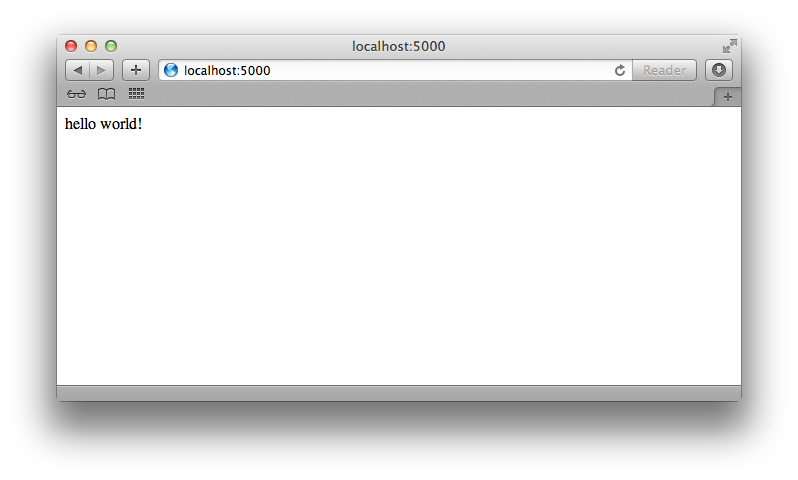
\includegraphics[width=0.8\textwidth]{images/flask-hello-napier.png}
\caption{Your first Python Flask web app.}
\label{fig:flask-hello-napier}
\end{figure}

\section{Wrapping Up}
\label{chapter_02_wrap-up}
\paragraph{} Right. Thats all the preliminaries in place for building web-apps in our learning environment. We can now run a small and lightweight, but otherwise similar to full Linux installs, virtualised server which will host our web-apps. We can log in to the server using SSH, navigate the Linux environment, and edit files using VIM. We can also take advantage of the installed Python language and Python-Flask web-app library to build our own web-apps.

\begin{framed}
\textbf{CHALLENGE} Create a Github or Bitbucket account. Bitbucket allows you to create an unlimited number of private repositories if you use your @napier address to register whereas Github restricts the number of private repos. That said, either site allows you to create as manay public repositories as you like. Create a remote repo in your Github or Bitbucket account called `set09103'. Run Levinux and log in then clone your set09103 repo. Create a new file in your repo called `hello.txt' and put the message ``Hello Simon'' in it then add, commit and push your changes to your remote repo. Once you have done this, check on either Github or Bitbucket to ensure that your text file is in the repo where you expect it to be then send an email to Simon containing the name of your account, which service, Github or Bitbucket, you are using, and the clone url for your set09103 repository. {\emph{If you use a private repository then you will have to add my account as a collaborator. On both Github and Bitbucket my account name is `siwells'}}. I will then pull everyone's repos to ensure that we are all at the same place in our learning. We will then use the set09103 repos as the place to store our coursework projects and for the hand-in. This just means that we have everything in place early before the hand-in deadline.
\end{framed}

\paragraph{} Over the next few chapters we will look at a whole host of things we can do with Flask. However you should also rest assured that all of the tools we are learning will prove useful to you at some point in your career and will help you to become the best developers that you can be.

%%%%%%%%%%%%%%%%%
%%%%%%%%%%%%%%%%%
% APPENDICES 
%%%%%%%%%%%%%%%%%
%%%%%%%%%%%%%%%%%

\appendix
\chapter{Cribsheets}
\label{cribsheets}
\paragraph{} These cribsheets are useful for collecting together lots of knew syntax but are no substitute for your own notes (and practise. Stuff you know is much better than stuff you can look up). Either way, as you learn new stuff you should expand these cribsheets with extra commands that you find useful.

\section{Linux}
\label{cribsheet_linux}

\subsection{Some useful aliases}

\begin{description}
\item[{\raise.17ex\hbox{$\scriptstyle\sim$}}] An alias that means your home directory within the filesystem hierarchy. In Levinux, for the user tc this would expand to /home/tc
\item[..] An alias that means the parent of the current directory
\end{description}

\subsection{Some useful commands}
\begin{description}
\item[cat \emph{filename}] Display the contents of the file \emph{filename}
\item[cd] Change to your home directory /home/tc or \textasciitilde/home
\item[cd \emph{..}] Change directory to the parent of the current directory
\item[cd \emph{directoryname}] Change directory to the named directory
\item[ls] List the names of the files in the current directory
\item[ls  \emph{directoryname}] List the contents of the named directory
\item[mkdir \emph{directoryname}] Create a new directory in the current directory
\item[pwd] Display the path to the current directory in the filesystem hierarchy, e.g. show you where you are relative to the root
\item[rm \emph{filename}] Delete the named file
\item[rm -rf \emph{directoryname}] Will delete the named directory and all of its contents
\item[touch \emph{filename}] Will create a new file called filename
\end{description}

\section{Vim}
\label{cribsheet_vim}
\begin{description}
\item[\$ vim] - Shell command to start a new unnamed empty document in Vim
\item[\$ vim filename.txt] - Shell command to open `filename.txt' in Vim. If it exists then the file will be opened, otherwise an empty file will be opened for editing that will be saved as `filename.txt' when you use the (w)rite command
\item[$<$ESC$>$] - Enter command Mode
\item[$<$ESC$>$i$<$ENTER$>$] Enter (i)nsert edit mode
\end{description}
\paragraph{} The following are a core set of Vim commands that are all used whilst in Command mode, e.g. after typing $<$ESC$>$
\begin{description}
\item[:q$<$ENTER$>$] - (q)uit
\item[:q!$<$ENTER$>$] - (q)uit and discard any changes
\item[:w$<$ENTER$>$] - (w)rite changes to file
\item[:wq$<$ENTER$>$] - (w)rite changes to file then (q)uit
\item[:e \emph{filename} $<$ENTER$>$] - Open file \emph{filename} in Vim for editing
\item[dd$<$ENTER$>$] - Delete the entire line that the cursor is on
\item[x$<$ENTER$>$] - Delete the character that the cursor is on
\item[j] - Move the cursor up one line (NB. You can also use the `up' arrow key
\item[k] -  Move the cursor down one line (NB. You can also use the `down' arrow key
\item[l] -  Move the cursor right one character (NB. You can also use the `right' arrow key
\item[h] -  Move the cursor left one character (NB. You can also use the `left' arrow key
\item[gg] -  Go to start of file	 
\item[G] - Go to end of file
\item[\$] - Move cursor to the end of the current line
\item[0] - Move cursor to start of current line (NB. Thats a zero)
\item[$<$CTRL$>$e] - Scroll up
\item[$<$CTRL$>$y] - Scroll down	
\item[$<$CTRL$>$b] - Page Up	
\item[$<$CTRL$>$f] - Page Down
\item[/\emph{search-term}] - Search forward for `search-term' in the current file (Use `n' for (n)ext match in current direction and (N) for next match in opposite direction)
\item[?\emph{search-term}] - Search backward for `search-term' in the current file (Use `n' for (n)ext match in current direction and (N) for next match in opposite direction)
\item[u] - Undo the last command
\item[.] - Repeat the last command
\end{description}

\paragraph{} Vim has many more commands and many ways in which individual commands can be composed into more complex composite commands. We've seen above a core set of essential commands, now we'll have a smattering of interesting further commands that are useful when editing and will give you a flavour of what Vim has to offer:
\begin{description}
\item[J] - Combine (``join'') next line with this one
\item[nG] - Move cursor to line n, e.g. 1G will take you to the first line of the file
\item[ma] - Mark current position
\item[d`a] - Delete everything from the marked position to here
\item[`a] -  Go back to the marked position] 
\item[:s/s1/s2] - Replace (``substitute'') (the first) s1 in this line by s2
\end{description}

\chapter{Annotated Code Examples}
\label{annotated}

\section{Python Flask `Hello Napier'}
\label{annotated_hello_napier}
\paragraph{} An annotated walk through the code from hello.py that we saw in section \ref{python-flask}.

\begin{lstlisting}
from flask import Flask 
app = Flask(__name__)

@app.route("/")
def hello():
    return "Hello Napier!"

if __name__ == "__main__":
    app.run(host='0.0.0.0')

\end{lstlisting}

\begin{description}
\item[Line 1] \emph{from flask import Flask}\\ 
Import the Flask class from the flask library. The library contains pre-written code and utilities that are useful when writing a web-app. In this case an instance of the Flask class will be our WSGI application.
\item[Line 2] \emph{app = Flask(\_\_name\_\_)}\\
Create an instance of the Flask class. The argument `\_\_name\_\_' is the name of the flask applications module. This is used to help flask to find resources relative to the Python module such as static web resources like image files, templates, or CSS. We also create a variable, `app', that references the newly instantiated Flask class so that we can use it later.
\item[Line 4] \emph{@app.route("/")}\\
Lines that start with @ in Python are decorators. In this case we use the route() decorator to tell Flask which URL should trigger the function that route() decorates, e.g. when a browser hits the root of the url, `/' then the hello() function is run. We use route() decorators in flask to build up our HTTP API that a browser can retrieve.
\item[Line 5] \emph{def hello():}\\
This defines a function called `hello()'. hello() is executed whenever someone requests the root url.
\item[Line 6] \emph{return "Hello Napier!"}\\
All our hello() does is to return the string ``Hello Napier''. It is this string that is displayed in the browser. We could instead return some HTML for a richer experience but plain textis sufficient for now.
\item[Line 8] \emph{if \_\_name\_\_ == "\_\_main\_\_":}\\
This is used to control how the Python module and the flask app server is run. We only want to use app.run() if this script is executed from the Python interpreter, e.g. by calling \$python hello.py. If we were to use an app server instead then the app.run() would be performed differently.
\item[Line 9] \emph{app.run(host='0.0.0.0')
}\\
Calls the run() function of the Flask app class instance to start our development server running using this app as the web app. This line also tells the app to run on a network interface that is accessible from an external address, e.g. from the Windows machine that is running Levinux, otherwise our app would only be accessible within Levinux and we don't have a graphical browser installed there.
\end{description}

\backmatter

\bibliographystyle{plain}

\bibliography{adv-web-tech}

\end{document}

